\newpage
\section{Tree-to-model transformation with TGGs}
\genHeader

Our goal in this section is to break down the \texttt{MocaTree} to \texttt{Dictionary} transformation into smaller, modular steps. More precisely, we
want separate rules for transforming a \texttt{Folder} into its appropriate container element (i.e., \texttt{Library} or \texttt{Shelf}), then individual rules
to handle whatever \texttt{File} and \texttt{Node} elements they contain.

\vspace{0.5cm}

Let's briefly look at the models we'll be working with. We start with Fig.~\ref{eclipse:treeStart},\footnote{You can view this model in your Eclipse editor by
placing the contents of \texttt{tree.xmi} into eMoflon's Graph Viewer, as introduced in Part II, Section 4.} where our root input folder, \texttt{MyLibrary},
contains two subfolders with at least one dictionary \texttt{File} each. Each dictionary has one equivalent dictionary root \texttt{Node} with at least two
children representing the title and first \texttt{ENTRY}, along with an unknown number of additional nodes. Of the remaining nodes, there may be one that stores
the dictionary author's contact information. All the rest will be \texttt{ENTRY} nodes with two children representing its content and level information.

\vspace{1cm}

\begin{figure}[htbp]
\hspace{-1.5cm}
 	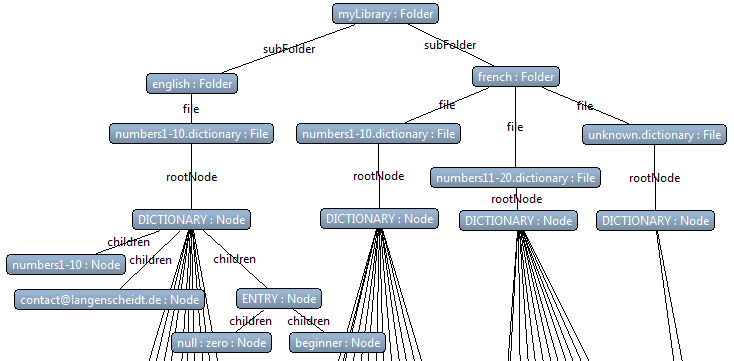
\includegraphics[width=1.2\textwidth]{eclipse_TreeStartMetamodel}
 	\caption{The \texttt{MocaTree} model of our input directory}
 	\label{eclipse:treeStart}
\end{figure}

\newpage

Our transformation intends to finish with a \texttt{Dictionary} model resembling Fig.~\ref{eclipse:dictionaryStart}, where the root \texttt{MyLibrary} node has
four subfolders, one for each shelf and author. These subfolders will likely pair up, sharing a child \texttt{Dictionary} element containing an unknown number
of entries.

\vspace{1cm}

\begin{figure}[htbp]
\hspace{-1.5cm}
    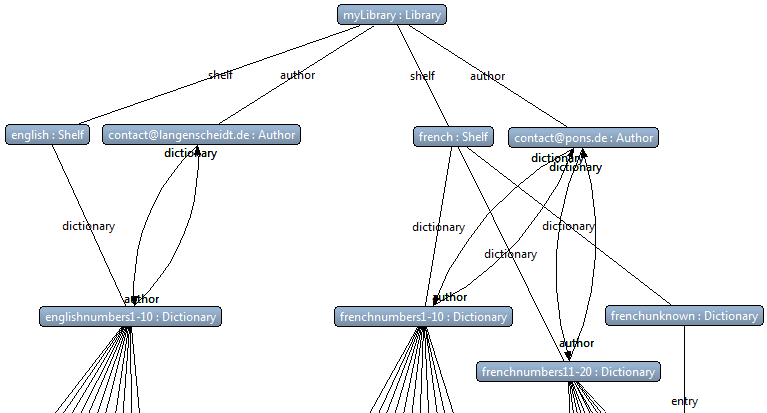
\includegraphics[width=1.2\textwidth]{eclipse_DictionaryResultMetamodel}
 	\caption{The final \texttt{Dictionary} target model}
 	\label{eclipse:dictionaryStart}
\end{figure}

\vspace{1cm}

As you can see, it's important to keep in mind the flexibility that the rules for this transformation will require. While our example model is small
enough to count the number of entries our rules will need to account for, future models may not be so forgiving. Just like SDM patterns, it's key to avoid
situation-specific TGG rules.

\jumpDual{treeToModel vis}{treeToModel tex}

\newpage
\hypertarget{treeToModel vis}{}
\subsection{The visual transformation rules}
\visHeader

\begin{itemize}

\item[$\blacktriangleright$] Expand the \texttt{<<Rules Package>>} node in EA and open the \texttt{Rules} diagram. Create a new rule named
\texttt{FolderToLibraryRule}, double-clicking the new element to open its diagram. Complete the rule as depicted in Fig.~\ref{ea:FolderIntoLibrary_Complete}.
Remember -- we established that first correspondence type when creating the TGG schema in Section 1.

\vspace{0.5cm}

\begin{figure}[htbp]
\begin{center}
  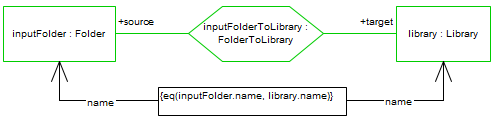
\includegraphics[width=0.8\textwidth]{ea_FolderToLibraryRule}
  \caption{completed folder into library}
  \label{ea:FolderIntoLibrary_Complete}
\end{center}
\end{figure}

\item[$\blacktriangleright$] We're able to use this entire rule as black context for the next rule in order to handle the creation of shelves. Select
\texttt{inputFolder, inputFolderToLibrary,} and \texttt{library}, then use the eMoflon control panel to \texttt{derive} a new rule. Name this \texttt{ForAllShelfRule}.

\item[$\blacktriangleright$] This will open a new diagram with three black objects, representing the context. This rule is remarkably similar to
\texttt{FolderToLibraryRule}, except it will need two green links connecting the new elements to their respective container. Complete \texttt{ForAllShelfRule}
as depicted in Fig.~\ref{ea:ForAllShelves_Complete}. You'll need to create a new correspondence type, \texttt{FolderToShelf} in either the schema (as we did
for \texttt{FolderToLibrary}) or by selecting \texttt{Create new Link} in the dialogue that appears from quick-linking between \texttt{shelfFolder} and
\texttt{shelf}.

\vspace{0.5cm}

\begin{figure}[htbp]
\begin{center}
  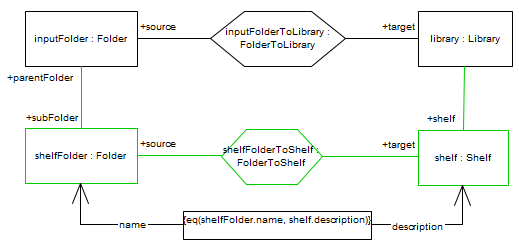
\includegraphics[width=0.8\textwidth]{ea_ForAllShelfRule}
  \caption{completed ForAllShelves}
  \label{ea:ForAllShelves_Complete}
\end{center}
\end{figure}

\newpage

\item[$\blacktriangleright$] Now we're able to handle the dictionary \texttt{File} elements. Ananlogously to how you began the previous rule, select
\texttt{shelfFolder}, \texttt{FolderToShelf}, and \texttt{shelf}, and derive \texttt{NodeToDictionaryRule}.

\item[$\blacktriangleright$] Build it as shown in Fig-~\ref{ea:NodeToDictionary_Complete}. As you can see, this rule creates a consistency between
\texttt{dictionaryNode} and the \texttt{dictionary} instance, and only handles the first \texttt{titleNode} in the tree structure. Nearly every element is
involved in order to correctly set the \texttt{dictionary} and \texttt{dictionaryFile} names in two different constraints!

\begin{figure}[htbp]
\begin{center}
  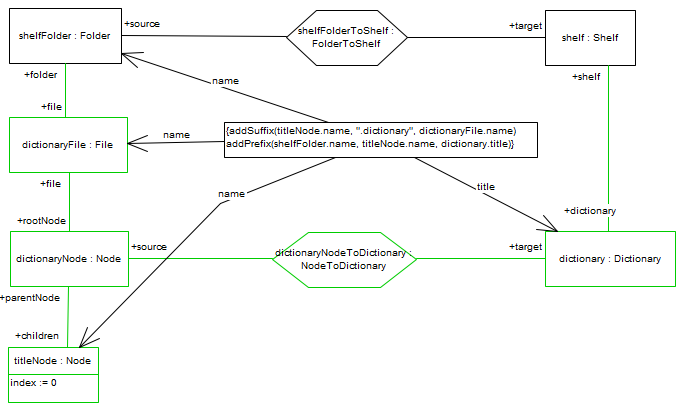
\includegraphics[width=\textwidth]{ea_NodeToDictionaryRule}
  \caption{completed NodeToDictionary}
  \label{ea:NodeToDictionary_Complete}
\end{center}
\end{figure}

\item[$\blacktriangleright$] Please note that the \texttt{index} \emph{attribute constraint} is required in order to ensure that the node with the title
information is correctly matched. We could have also included a \texttt{node} to handle the author, a third, fourth, or even tenth \texttt{node} connected to
\texttt{DictionaryNode}, but that would mean the pattern absolutely has to match to an author and ten elements, which may not always exist. Instead, we'll
create separate rules for each of these types which can be called as many times as necessary.

\item[$\blacktriangleright$] Let's handle the \texttt{entry} elements first. Create and complete \texttt{ForAllEntryRule} and depicted in
Fig.~\ref{ea:ForAllEntry_Complete}. We needed to match both a \texttt{contentNode} and \texttt{indexNode} to each \texttt{entryNode}, bound by their
\texttt{index} values in order to ensure the correct EString attributes were set to an \texttt{entry}'s \texttt{content} and \texttt{level} values.

\begin{figure}[htbp]
\begin{center}
  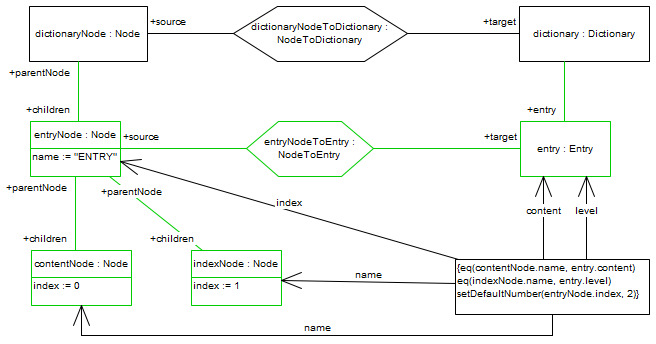
\includegraphics[width=\textwidth]{ea_ForAllEntryRule}
  \caption{completed ForAllEntry}
  \label{ea:ForAllEntry_Complete}
\end{center}
\end{figure}

\item[$\blacktriangleright$] Return to \texttt{NodeToDictionaryRule}. We need to think about what context elements we'll need for our next rule to handle
authors. Not only will we need \texttt{DictionaryNode} and \texttt{dictionary} as we did in \texttt{ForAllEntry}, we'll also need \texttt{shelf} and
\texttt{library} in order to satisfy the \texttt{Dictionary} metamodel, where each \texttt{author} is linked to both individual \texttt{dictionary} and
\texttt{library} elements. Derive and create \texttt{AuthorRule} as depicted below Fig.~\ref{ea:AuthorRule}

\begin{figure}[htbp]
\begin{center}
  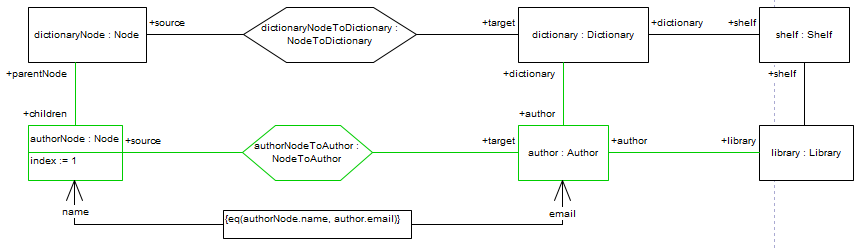
\includegraphics[width=\textwidth]{ea_AuthorRule}
  \caption{completed AuthorRule}
  \label{ea:AuthorRule}
\end{center}
\end{figure}

\item[$\blacktriangleright$] You're nearly done! Make sure everything is saved, and validate your TGG. If a dialogue appears saying the attempt was
unsuccessful, you may simply need to update your original schema diagram. To do so, open \texttt{dictionaryCodeAdapter}, right click anywhere in the diagram and
add any missing elements by navigating to ``Insert Existing Element'' (Fig.~\ref{ea:insertContext}), and selecting the missing correspondence types from the package's
tree (Fig.~\ref{ea:insertTree}).

\begin{figure}[htbp]
   \centering
      \subfloat[comment 1 \update]{
        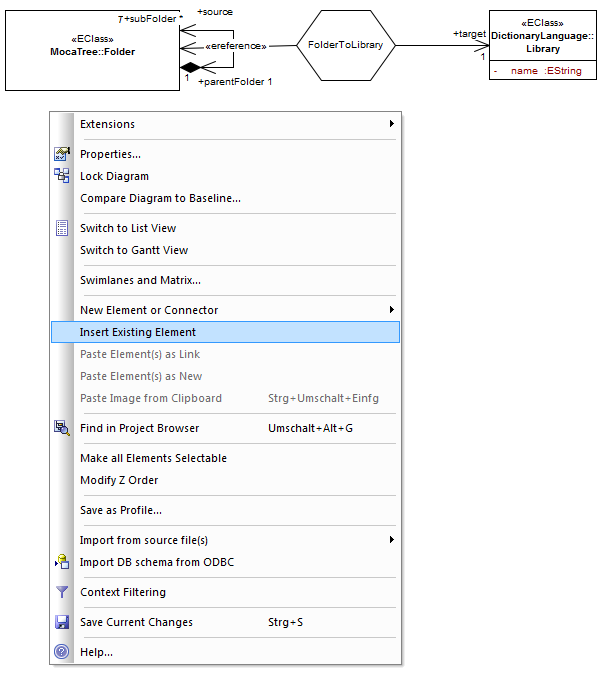
\includegraphics[width=0.45\textwidth]{ea_InsertExistingElements}
        \label{ea:insertContext}
      }
      \subfloat[Bugger. Comment 2]{
        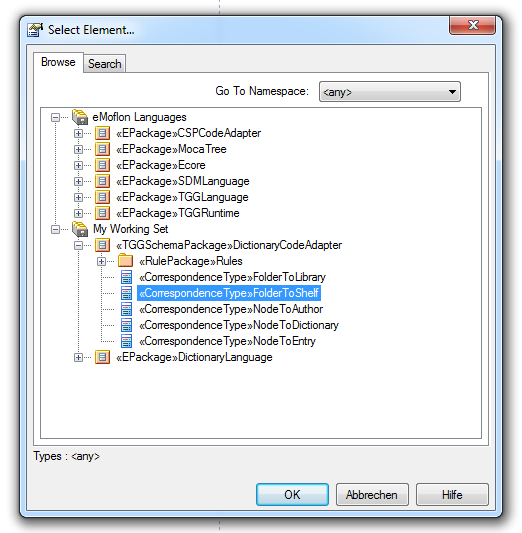
\includegraphics[width=0.45\textwidth]{ea_insertElementTree}
        \label{ea:insertTree}
      }
      \caption{Insert elements you created on the fly}
\end{figure}

\item[$\blacktriangleright$] Your schema diagram should come to resemble Fig.~\ref{ea:Schema_Complete}.

\begin{figure}[htbp]
\begin{center}
  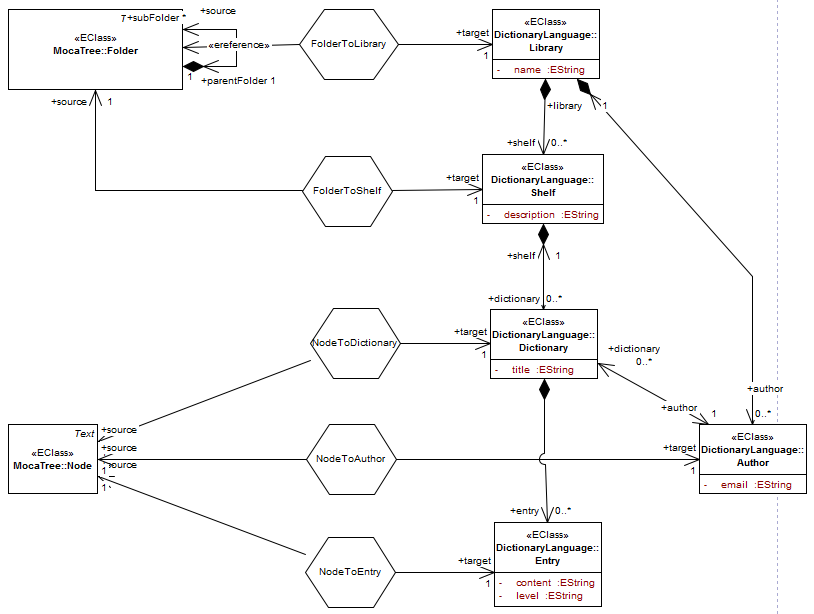
\includegraphics[width=\textwidth]{ea_finalSchema}
  \caption{completed Schema}
  \label{ea:Schema_Complete}
\end{center}
\end{figure}

Run TGG main -- two author nodes were created from
\texttt{numbers1-10.dictionary} and \texttt{numbers11-20.dictionary} having the same author. Having repeated, identical \texttt{author} elements may not always be desired. Wouldn't it sometimes be nice to have \emph{one} author can can be
connected to multiple \texttt{dictionary} elements?

\item[$\blacktriangleright$] We can use the basis of \texttt{AuthorRule} (return to this) for \texttt{ForAllNewAuthorRule} and \texttt{ExistingAuthorRule}. We
want to avoid copy and pasting where we can, but we need all the same elements. eMolfon's visual syntax has a cool \emph{refinement} feature, which enables you
to adjust only specific parts of an already created rule. First, return to the \texttt{Rules} diagram

\item[$\blacktriangleright$] Return to the main \texttt{Rules} diagram, and select \texttt{AuthorRule} and press \texttt{Alt + enter} to raise its properties
dialogue. Go to ``Properties/Details'' and select the \texttt{Abstract} box (Fig.~\ref{}).

\item[$\blacktriangleright$] Now create two new rules, \texttt{ForAllNewAuthorRule} and \texttt{ExistingAuthorRule}. Quick-link from each of them to
\texttt{AuthorRule} and select \texttt{Create Refinement Link}. Each of these now inherits the same pattern as \texttt{AuthorRule}.

\item[$\blacktriangleright$] Lets implement \texttt{ForAllNewAuthorRule}. Double-click its class and create a green \texttt{authorNode}, and black
\texttt{library} element. There's no need to worry about creating appropriate links; If you extend your imagination, picture this rule being placed on directly
on top of \texttt{AuthorRule}, like a clear cellophane sheet.\footnote{This may be easier to imagine if you place these objects in the same place as their
original}. While this rule doesn't actually modify anything from the original rule, this will make sense for the next rule.

\item[$\blacktriangleright$] Open the \texttt{ExistingAuthorRule} diagram. This time, we don't want to create an \texttt{authorNode}, but instead connect a
pre-existing \texttt{author} to \texttt{Library} (FIG). Compare this rule to its abstract.


\item[$\blacktriangleright$] Fantastic work: your forward transformation is now completed with TGGs. Try validating and exporting your package to Eclipse. If it
doesn't work at first, and everything has been done correctly, you may have to update the schema file -- it may be missing some elements you created on the fly.
Add any missing elements (it should resemble FIG), then validate again. Once it succeeds, refresh your Eclipse workspace to generate the corresponding code.


\jumpSingle{t2m close}

\end{itemize}


\newpage
\hypertarget{treeToModel tex}{}
\subsection{The textual transformation rules}
\texHeader

Please note that we have assumed a basic understanding of TGGs, specifically those about constructing each scope in a rule, and how to use Eclipse efficiently
with eMoflon's auto-completion feature. If you find this section challenging, we recommend first working through Part IV to cover TGG fundamentals.

\begin{itemize}

\subsubsection{FolderToLibraryRule} % ---------------------------------

\item[$\blacktriangleright$] Return and expand the \texttt{DictionaryCodeAdapter} TGG package and right-click on the \texttt{Rules} folder. Create your first
rule by navigating to ``New/TGG Rule," naming it \texttt{Folder\-To\-Lib\-rary\-Rule}.

\item[$\blacktriangleright$] All this rule needs to do is create a \texttt{Folder} (i.e., ``myLibrary'') together with its equivalent \texttt{Library}, and
establish a correspondence link between them. Edit your rule until it resembles Fig.~\ref{eclipse:FolderToLibraryRule}.

\vspace{0.5cm}

\begin{figure}[htbp]
\begin{center}
  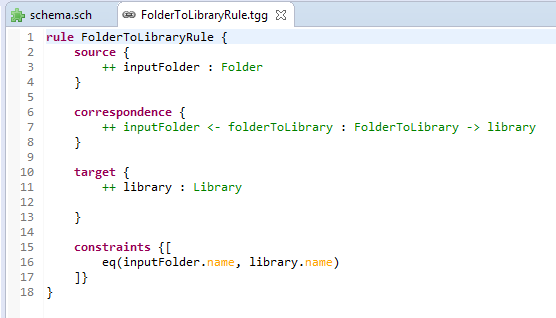
\includegraphics[width=\textwidth]{eclipse_FolderToLibraryRule}
  \caption{The TGG transformation begins with this rule.}
  \label{eclipse:FolderToLibraryRule}
\end{center}
\end{figure}

\vspace{-0.5cm}

\subsubsection{ForAllShelfRule} % ---------------------------------

\item[$\blacktriangleright$] Let's use some elements from the previous rule to help us define how to handle creating shelves for our library. Copy and paste the
required context elements from \texttt{FolderToLibraryRule} in a new \texttt{ForAllShelfRule}, adding a new \texttt{shelfFolder} and \texttt{shelf} as depicted
in Fig.~\ref{eclipse:ForAllShelvesRule}.

\vspace{0.5cm}

\begin{figure}[htbp]
\begin{center}
  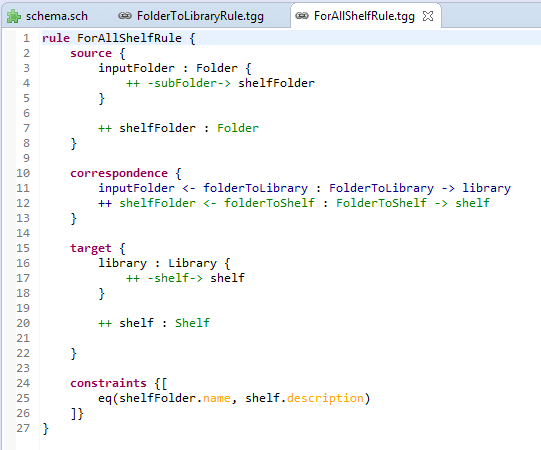
\includegraphics[width=0.9\textwidth]{eclipse_ForAllShelfRule}
  \caption{\texttt{ForAllShelfRule}}
  \label{eclipse:ForAllShelvesRule}
\end{center}
\end{figure}

\item[$\blacktriangleright$] Add the new correspondence type to your \texttt{schema} (Fig.~\ref{eclipse:updatedSchema}).

\vspace{0.5cm}

\begin{figure}[h!]
\begin{center}
  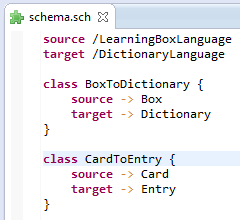
\includegraphics[width=0.7\textwidth]{eclipse_updatedSchema}
  \caption{Updated TGG \texttt{schema}}
  \label{eclipse:updatedSchema}
\end{center}
\end{figure}

\newpage

Now that we can assume the primary library and shelf containers exist, we can handle the dictionary \texttt{File} elements. We know from our generated
tree model that a dictionary will always have a title node, but we're unsure if an author will be included, and there's no way to know how many entries are
involved. Therefore, we should create at least three different rules to handle this stage of the transformation. 

\subsubsection{NodeToDictionaryRule} % ---------------------------------

\item[$\blacktriangleright$] Create a rule named \texttt{NodeToDictionaryRule} as indicated in Fig.~\ref{eclipse:NodeToDictionaryRule}.

\vspace{0.5cm}

\begin{figure}[htbp]
\begin{center}
  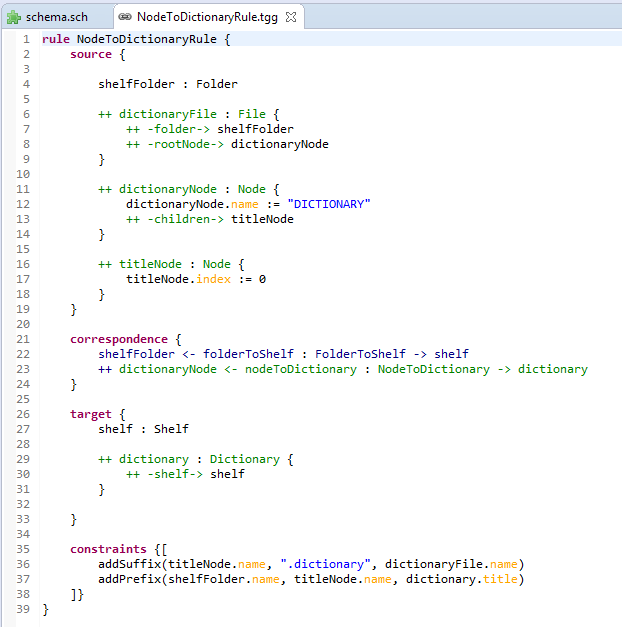
\includegraphics[width=\textwidth]{eclipse_NodeToDictionaryRule}
  \caption{\texttt{NodeToDictionaryRule} handling only \texttt{titleNode}s}
  \label{eclipse:NodeToDictionaryRule}
\end{center}
\end{figure}

\newpage

\item[$\blacktriangleright$] As you can see, this rule demands that a \texttt{shelfFolder} and \texttt{shelf} already exist before executing, implying that this
rule can only be called after executing \texttt{ForAllShelfRule}. An attribute constraint is used with \texttt{titleNode} to ensure that the correct child
\texttt{Node} is matched from \texttt{dictionaryNode}, and not accidentally to an author or entry node, which will have different indices.

\item[$\blacktriangleright$] This rule also imposes two constraints for attribute manipulation. We need to add the name of the shelf as a prefix to the title
node's name to get the dictionary's title (i.e., ``english'' + ``numbers1-10''). Similarly, the second constraint appends \texttt{.dictionary} to
\texttt{titleNode.name} to get the file name of the dictionary.

\subsubsection{ForAllEntryRule} % ---------------------------------

\item[$\blacktriangleright$] Let's handle \texttt{Entry} elements next. Create \texttt{ForAllEntryRule} so that it closely resembles
Fig.~\ref{eclipse:ForAllEntryRule}.

\vspace{0.5cm}

You can see that this rule has three attribute constraints, one of which we haven't encountered before. The first two \texttt{eq} constraints guarantee that
an \texttt{entryNode}'s content and index values remain consistent with its equivalent \texttt{entry} in a \texttt{dictionary}. The final constraint is to
ensure that any new \texttt{entryNode}s created in the backward transformation have index values set to 2. 

\vspace{0.5cm}

Without this final constraint, all new \texttt{entryNodes} would have a default 0 index value, and
could be mistaken as \texttt{titleNodes} as described in the previous \texttt{NodeToDictionaryRule}, causing the entire transformation to fail.

\newpage

\begin{figure}[htbp]
\begin{center}
  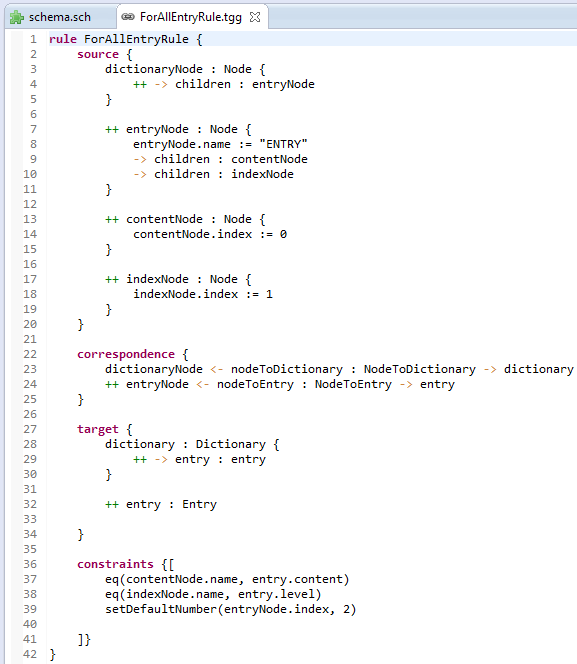
\includegraphics[width=\textwidth]{eclipse_ForAllEntryRule}
  \caption{\texttt{ForAllEntryRule}}
  \label{eclipse:ForAllEntryRule}
\end{center}
\end{figure}

\vspace{0.5cm}

The last thing we need to specify is how to handle \texttt{author}s. Transforming an \texttt{authorNode} to an \texttt{author} isn't as simple as
an \texttt{entryNode}, where you create an \texttt{entry} every time. Instead, we have to account for the possibility of a single author
for multiple dictionaries in a \texttt{Library}. While some users may not care about having redundant information, why not also provide a rule for users
who want to enforce unique authors in a \texttt{Library}?

\subsubsection{NewAuthorRule} % ---------------------------------

\item[$\blacktriangleright$] Create \texttt{NewAuthorRule}, and complete it as depicted in Fig.~\ref{eclipse:ForAllNewAuthorRule}. This is a one-to-one
correspondence rule, where every \texttt{authorNode} creates a new \texttt{author}. If this rule is used in a transformation, one might end up with
multiple authors with the same email address.

\vspace{0.5cm}

\begin{figure}[htbp]
\begin{center}
  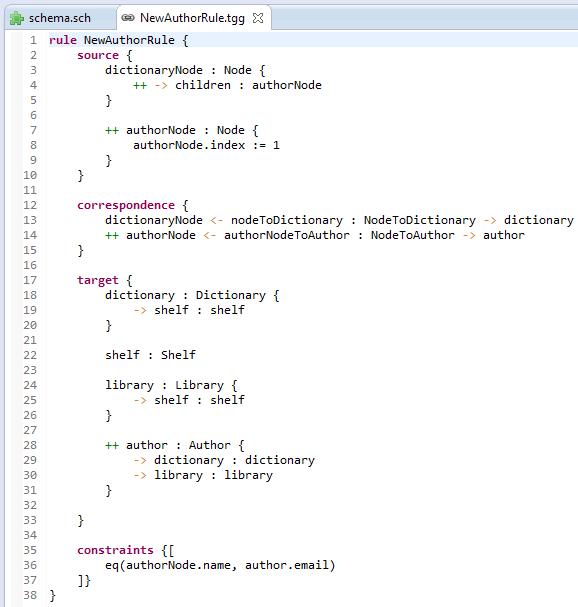
\includegraphics[width=\textwidth]{eclipse_NewAuthorRule}
  \caption{Creating new authors in \texttt{NewAuthorRule}}
  \label{eclipse:ForAllNewAuthorRule}
\end{center}
\end{figure}

\newpage

\subsubsection{ExistingAuthorRule} % ---------------------------------

\item[$\blacktriangleright$] Similarly, create \texttt{ExistingAuthorRule} as specified in Fig.~\ref{eclipse:ForExistingAuthorRule}. You should be able to
copy and paste the majority of the previous rule. In fact, the only thing you need to change are two small characters in front of \texttt{author} and its
\texttt{dictionary} reference, forcing the rule to find an existing \texttt{author}, if possible.

\vspace{0.5cm}

\begin{figure}[htbp]
\begin{center}
  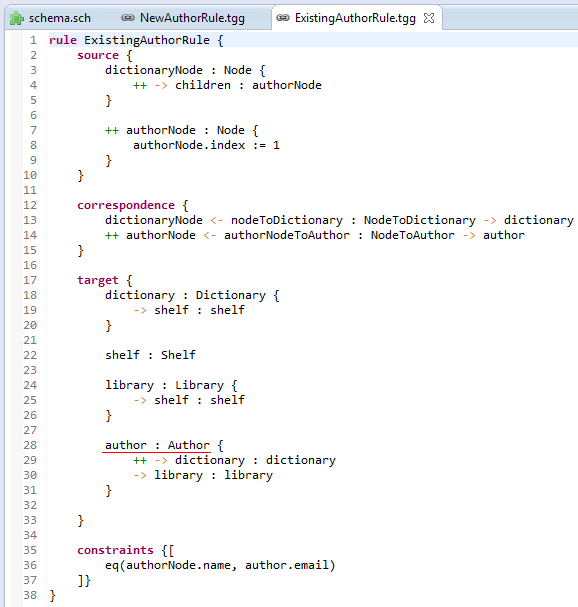
\includegraphics[width=\textwidth]{eclipse_ExistingAuthorRule}
  \caption{Checking for existing authors in \texttt{ExistingAuthorRule}}
  \label{eclipse:ForExistingAuthorRule}
\end{center}
\end{figure}

\newpage

\item[$\blacktriangleright$] Great work! You have now specified five different rules to handle a bidirectional text-to-model transformation! For confirmation,
your final schema and package explorer should now resemble Fig.~\ref{eclipse:schemaFinal}.

\vspace{0.5cm}

\begin{figure}[htbp]
\begin{center}
  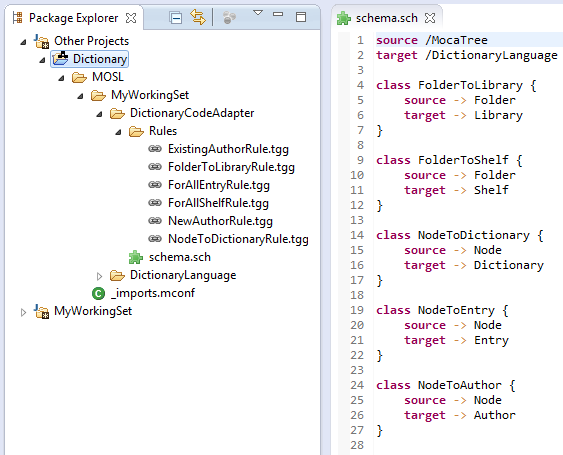
\includegraphics[width=\textwidth]{eclipse_finalSchema}
  \caption{Your final \texttt{rules} project structure and \texttt{schema}}
  \label{eclipse:schemaFinal}
\end{center}
\end{figure}

\vspace{0.5cm}

\item[$\blacktriangleright$] Given that everything has been done correctly, and MOSL hasn't reported any errors, build your TGG transformation. If problems
arise, be sure to double-check your files for spelling or other mistakes.

\end{itemize}


\newpage
\hypertarget{t2m close}{}
\subsection{Tree To Model Close}
\genHeader

\begin{itemize}

\item[$\blacktriangleright$] Navigate to ``src/org.moflon.tie'' right click and run TGGMain as application.

\begin{figure}[htbp]
\begin{center}
  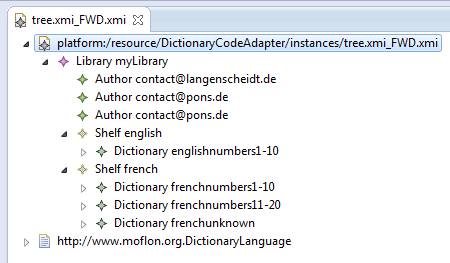
\includegraphics[width=0.7\textwidth]{eclipse_generatedForwardTransformation}
  \caption{completed forward transformation}
  \label{eclipse:generatedFwdTrsfm}
\end{center}
\end{figure}

\item[$\blacktriangleright$] Awesome, it works BEAUTIFULLY! Lets examine the output, \texttt{tree.xmi\_FWD.xmi} a little closer.

\item[$\blacktriangleright$] If you haven't already, read Section 6 from Part IV to learn how eMoflon's integrator feature can help you visualize how this
transformation was completed. Run the integrator on \texttt{corr\_FWD.xmi} until you reach the first (english) author node (do this as proof).

\begin{figure}[htbp]
\begin{center}
  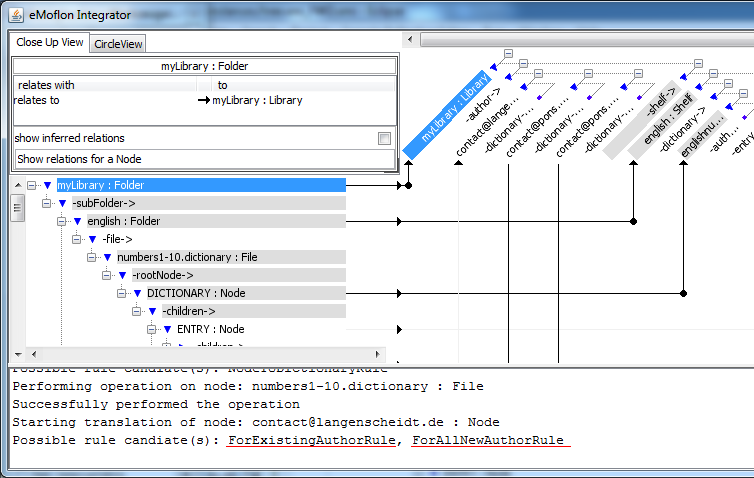
\includegraphics[width=0.7\textwidth]{eclipse_integratorAuthorChoice}
  \caption{completed forward transformation}
  \label{eclipse:generatedFwdTrsfm}
\end{center}
\end{figure}

\item[$\blacktriangleright$] The transformation decided to take one rule - either create or use existing - based on a random choice. The current set up isn't
dependable. We need to force a decision.

\item[$\blacktriangleright$] It had two choices and picked on at random. If you DO want to force a decision. You have two choices: ``I
don't care, \emph{always} make an author'' (duplicates), or no, ``I \emph{never} want there to be two of the same authors for one library.'' There are two ways
to define this: (Discuss options here?)

\end{itemize}

\begin{description}

\item[option1: Run-time] Create a configuration file for your TGG;

First: define \texttt{AuthorConfiguator}. FIG. put in in the same pacakage as your TGG. Don't make errors.

\begin{figure}[htbp]
\begin{center}
  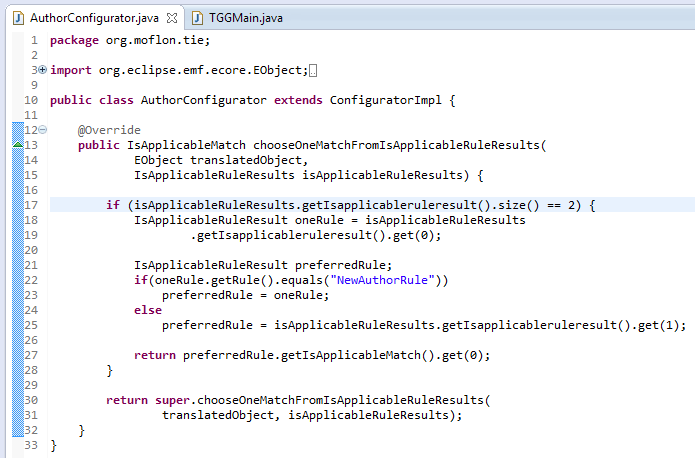
\includegraphics[width=0.7\textwidth]{eclipse_authorConfigurator}
  \caption{comment}
  \label{eclipse:authorConfig}
\end{center}
\end{figure}

Second: call it from \texttt{TGGMain}. FIG. Only need it in the forward transformation, so only put it once\ldots

\begin{figure}[htbp]
\begin{center}
  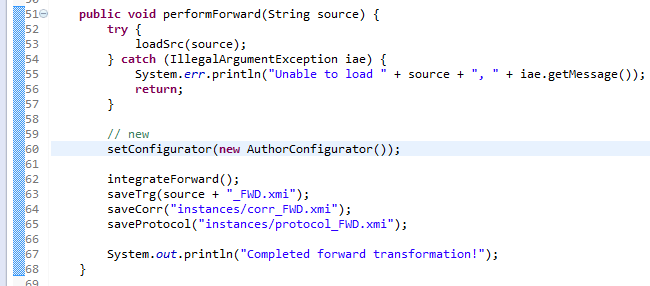
\includegraphics[width=0.7\textwidth]{eclipse_editTGGMain}
  \caption{comment on the edit}
  \label{eclipse:editTGGMain}
\end{center}
\end{figure}

\item[option2: Design-time] Create a NAC in \texttt{ForAllNewAuthors}; force it to skip
\hyperlink{NAC vis}{link1: {\bf VISUAL}}
\hyperlink{NAC tex}{link2: {\bf TEXTUAL}}

\hypertarget{NAC vis}{}
\subsubsection{VISUAL NAC}
\texHeader

\begin{itemize}

\item[$\blacktriangleright$] Add the following to \texttt{NewAuthor}

\begin{figure}[htbp]
\begin{center}
  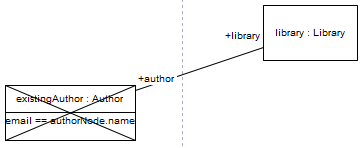
\includegraphics[width=0.7\textwidth]{ea_existingAuthorNAC}
  \caption{comment}
  \label{ea:existingAuthorNAC}
\end{center}
\end{figure}

\end{itemize}


\hypertarget{NAC tex}{}
\subsection{TEXTUAL NAC}
\texHeader

\begin{itemize}

\item[$\blacktriangleright$] Re-open \texttt{ForAllNewAuthor}. Add a NAC below \texttt{library} as depicted in FIG. If we had \emph{just} the library link,
then this rule would fail if the library had \emph{any} authors already set. So intead, we must add the email attribute constraint to match.

\begin{figure}[htbp]
\begin{center}
  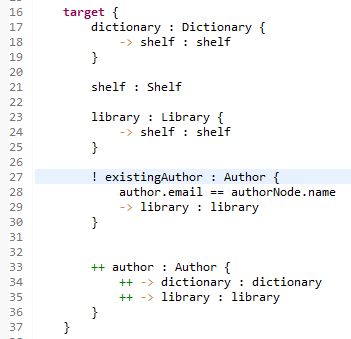
\includegraphics[width=0.7\textwidth]{eclipse_targetNAC}
  \caption{comment}
  \label{eclipse:existingAuthorNAC}
\end{center}
\end{figure}

\end{itemize}


\end{description}

% Back together, run TGGMain again
\newpage
\begin{itemize}

\item[$\blacktriangleright$] With your forced set up now constructed, Run TGGMain again. Use the integrator once more to see how it consistently chose your
decision.

\item[$\blacktriangleright$] Great work! You have now completed the first half of the complete round trip transformation, from Text to Model!

\end{itemize}

